\chapter{Capítulo de Ejemplo}

\section{Figuras, tablas y algoritmos}

\label{sec:figuras-tablas-algoritmos}
\subsection{Figuras}
Ejemplo de como hacer figuras utilizando el paquete figure\footnote{http://en.wikibooks.org/wiki/LaTeX/Floats,\_Figures\_and\_Captions} de LaTex.
\begin{figure}[!htbp]
    \centering
    
\includegraphics[width=0.5\textwidth]{capitulo-ej/graphics/latex.jpg}
    \caption{\label{fig:figura-ejemplo}Ejemplo de una figura en LaTex.}

\end{figure}

\begin{figure}[!htbp]
    \centering
    \begin{subfigure}[b]{0.45\textwidth}
            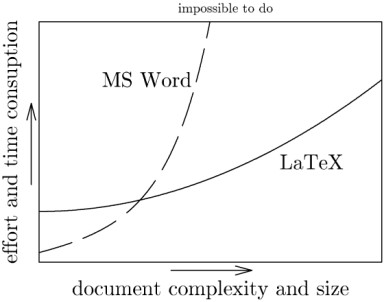
\includegraphics[width=\textwidth]{capitulo-ej/graphics/ejemplo-1.jpg}
            \caption{Subfigura 1.}
    \end{subfigure}
    ~~~~
    \begin{subfigure}[b]{0.45\textwidth}
            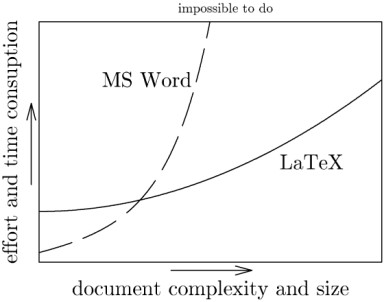
\includegraphics[width=\textwidth]{capitulo-ej/graphics/ejemplo-1.jpg}
            \caption{Subfigura 2.}

    \end{subfigure}
    \begin{subfigure}[b]{0.45\textwidth}
            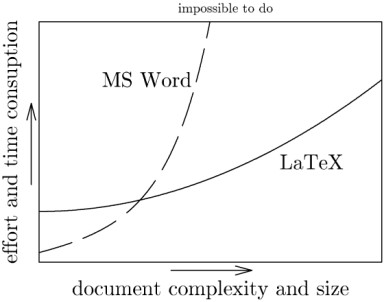
\includegraphics[width=\textwidth]{capitulo-ej/graphics/ejemplo-1.jpg}
            \caption{Subfigura 3.}
    \end{subfigure}
    ~~~~
    \begin{subfigure}[b]{0.45\textwidth}
            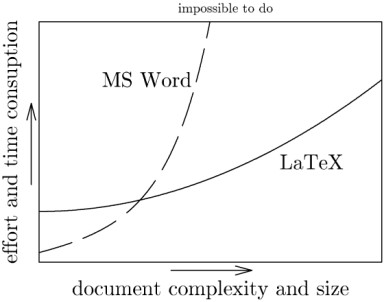
\includegraphics[width=\textwidth]{capitulo-ej/graphics/ejemplo-1.jpg}
            \caption{Subfigura 4.}

    \end{subfigure}
    \caption{\label{fig:ejemplo-fig-grilla}Ejemplo de una grilla de figuras en LaTex.}

\end{figure}

\subsection{Tablas}
Ejemplo de como hacer tablas utilizando el paquete table\footnote{http://en.wikibooks.org/wiki/LaTeX/Tables} de LaTex.
\begin{table}[!htpb]
    \begin{minipage}{\textwidth}
        \begin{center}
        \caption{\label{tab:tabla-ejemplo} Ejemplo de una tabla en LaTex.}
        \begin{tabular}{p{3cm} c c c c}
            \hline\\
            Año & Periodo & Columna & Columna2 & Columna3\\
            \hline
            \hline\\
            2014 & 29-12-13 / 31-05-14 & 10541 & 1052 & 2\\
            2013 & 30-12-12 / 21-12-13 & 153793 & 131306 & 70\\
            2012 & 01-01-12 / 22-12-12 & 37815 & 30588 & 11\\
            2011 & 03-01-11 / 29-12-11 & 53397 & 42264 & 62\\
            2010 & 11-10-09 / 25-12-10 & 21951 & 13760 & --$^a$\\
        \end{tabular}
        \footnotetext[1]{Esta es una nota.}
        \end{center}
    \end{minipage}
\end{table}

\subsection{Algoritmos}
Ejemplo de como hacer agloritmos utilizando el paquete algorithm\footnote{http://en.wikibooks.org/wiki/LaTeX/Algorithms} de LaTex.
\begin{algorithm}                      % enter the algorithm environment
\caption{Calculate $y = x^n$}          % give the algorithm a caption
\label{alg:alg1}                       % and a label for \ref{} commands later in the document
\begin{algorithmic}                    % enter the algorithmic environment
    \REQUIRE $n \geq 0 \vee x \neq 0$
    \ENSURE $y = x^n$
    \STATE $y \Leftarrow 1$
    \IF{$n < 0$}
        \STATE $X \Leftarrow 1 / x$
        \STATE $N \Leftarrow -n$
    \ELSE
        \STATE $X \Leftarrow x$
        \STATE $N \Leftarrow n$
    \ENDIF
    \WHILE{$N \neq 0$}
        \IF{$N$ is even}
            \STATE $X \Leftarrow X \times X$
            \STATE $N \Leftarrow N / 2$
        \ELSE[$N$ is odd]
            \STATE $y \Leftarrow y \times X$
            \STATE $N \Leftarrow N - 1$
        \ENDIF
    \ENDWHILE
\end{algorithmic}
\end{algorithm}

\subsection{Ecuaciones}
En esta sección se añade una pequeña ecuación con el fin de ejemplificar su
uso \addsymbol{symbol:x} \addsymbol{symbol:a_i}.
\begin{equation}\label{eq:ecuacion-ej}
  x = a_0 + \cfrac{1}{a_1
          + \cfrac{1}{a_2
          + \cfrac{1}{a_3 + \cfrac{1}{a_4} } } }
\end{equation}

\section{Referencias y citaciones}
Para referenciar secciones, figuras, tablas, algoritmos, o formulas se puede
emplear $\setminus$ref\{label-del-item\} o emplear cualquiera de las sigientes macros:


\begin{itemize}
\item $\setminus$secref\{label-sec\} : Ejemplo \secref{sec:figuras-tablas-algoritmos}
\item $\setminus$tabref\{label-tab\} : Ejemplo \tabref{tab:tabla-ejemplo}
\item $\setminus$figref\{label-fig\} : Ejemplo \figref{fig:ejemplo-fig-grilla}
\item $\setminus$algref\{label-alg\} : Ejemplo \algref{alg:alg1}
\item $\setminus$eqref\{label-eq\} : Ejemplo \eqref{eq:ecuacion-ej}
\end{itemize}

En esta sección se añade un ejemplo de como citar a un autor, utilizando
el $\setminus$cite\{label-bib1\} de bibText \footnote{http://en.wikibooks.org/wiki/LaTeX/Bibliography\_Management}.
Por ejemplo esta es una citación \cite{griffiths1997learning} a un solo
autor, y esta es a 2 autores \cite{griffiths1997learning, lamport1985i1}.
